\documentclass[a4paper, 11pt]{book}
\usepackage{CJKutf8}
\usepackage{graphicx}
\usepackage{indentfirst}
\usepackage[T1]{fontenc}
\usepackage{lmodern}
\usepackage{setspace}
\addtolength{\parskip}{3pt}
\linespread{1.3} %一倍半行距
\begin{CJK*}{UTF8}{bsmi}
\renewcommand\tableofcontents{目錄}
\renewcommand\listoffigures{圖片目錄}
\renewcommand\listoftables{圖表目錄}
\renewcommand\figurename{圖}
 \setlength{\parindent}{2em}
    \title{\Huge\textbf{中國數學家}}
    \author{\textsc{武國寧}}
\begin{document}
\frontmatter
\maketitle

\tableofcontents
\listoffigures
\listoftables
\graphicspath{./Figs/}


\mainmatter

\chapter*{引言}

\chapter*{李善蘭}

\begin{figure}[htbp]
    \centering
    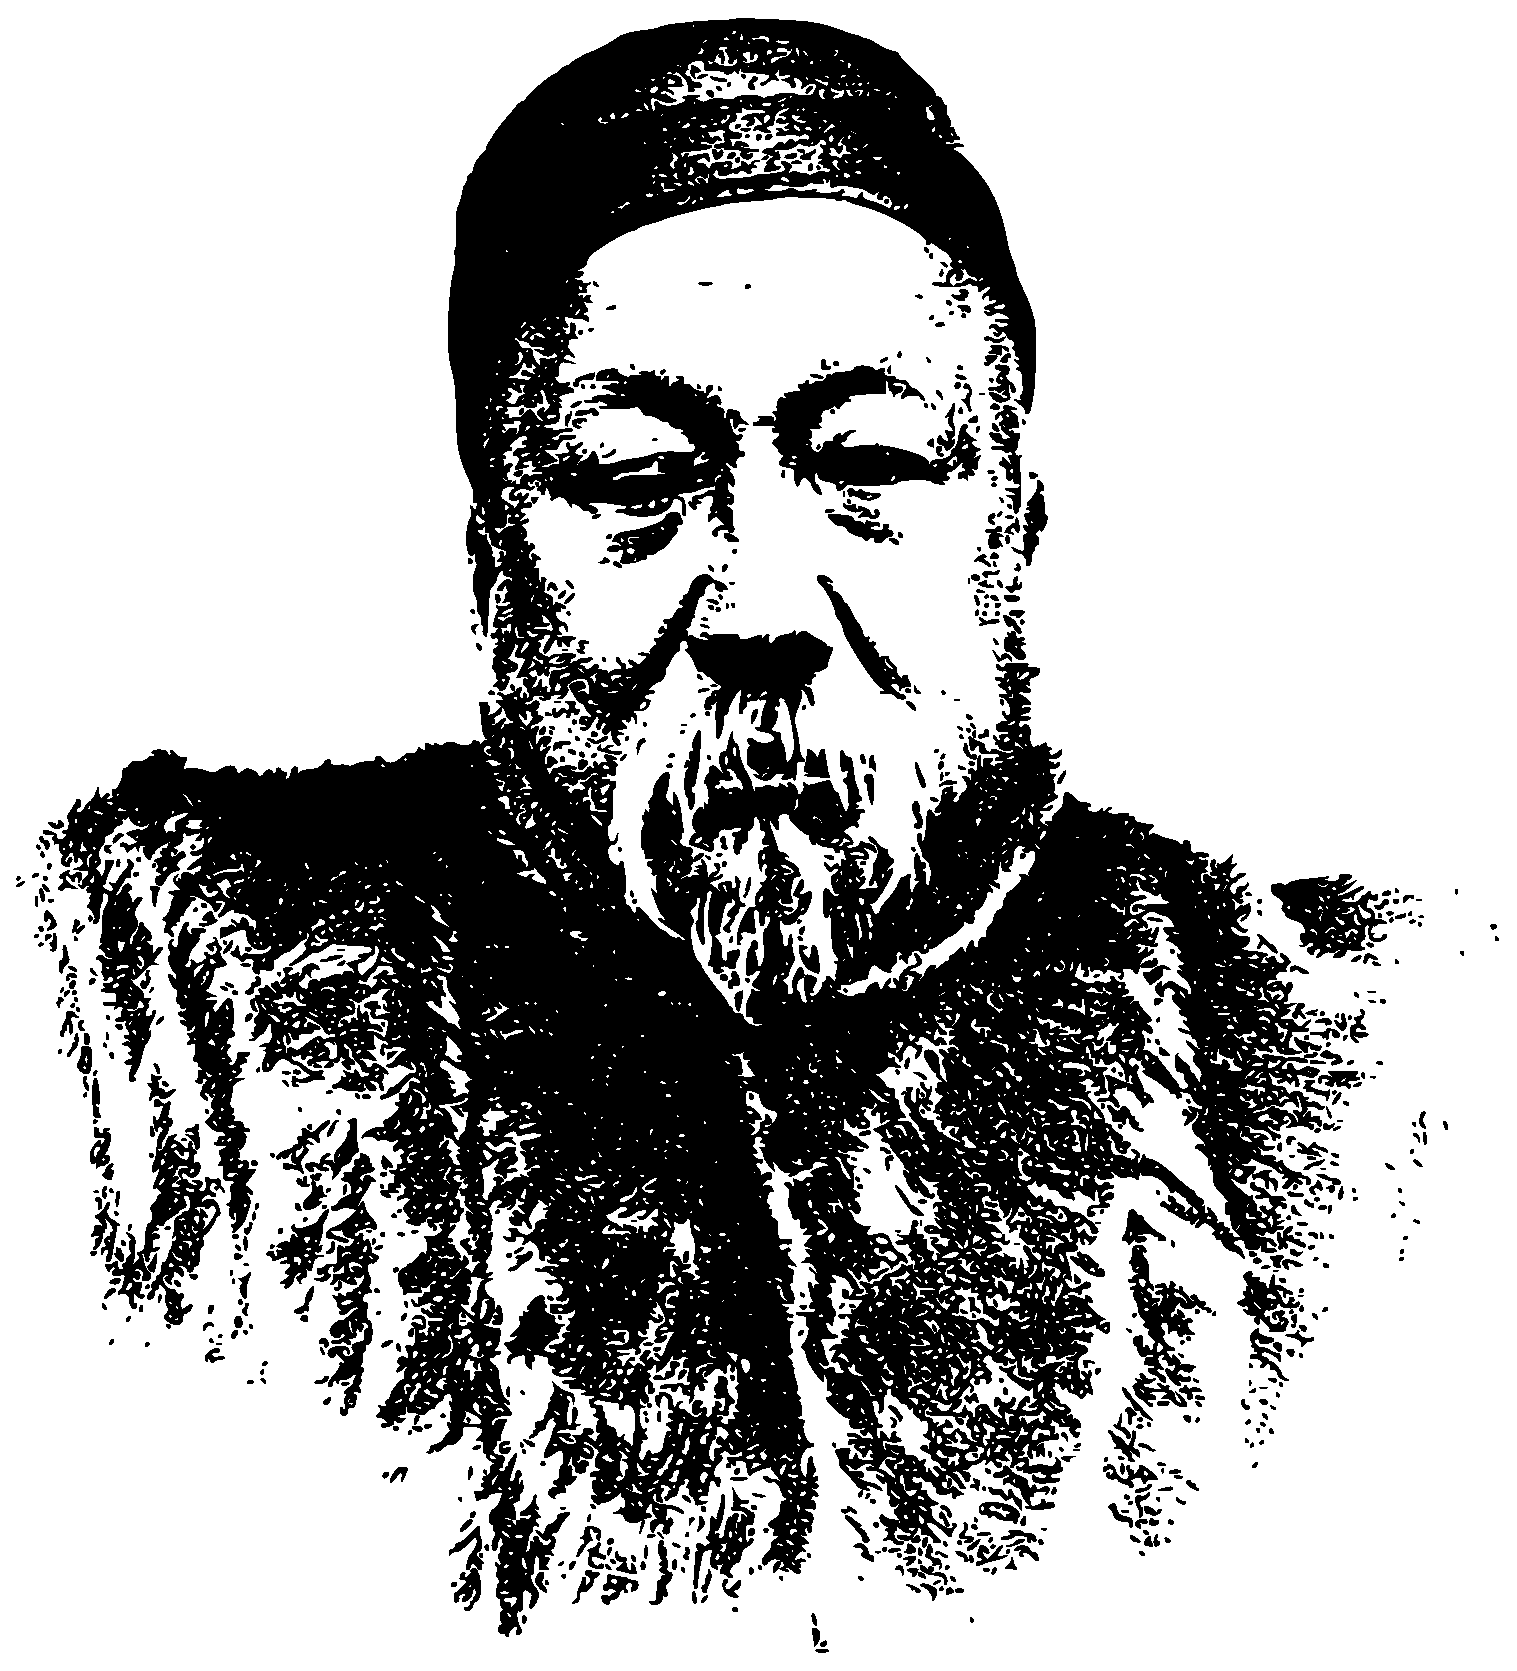
\includegraphics[width=6cm, height=8cm]{./Figs/Li_Shanlan.eps}
    \label{fig:Li_Shanlan}
    \caption{李善蘭}
\end{figure}
    李善蘭(1810年-1882年)字壬叔,號秋紉,中國清朝數學家。
    浙江省杭州府海寧縣人。為清代數學史上的傑出代表,中國近代數學的先驅。
    通詩文,曾幫基督教傳教士翻譯聖經。
    
\section*{生平}

\indent
李善蘭於清嘉慶十五年(1810年)1月2日生於浙江海寧縣硤石鎮。10歲即通《九章算術》,
15歲通習《幾何原本》六卷,17歲參加杭州鄉試未中。道光二十五年(1845年)以所著
《四元解》二卷呈浙江名士顧觀光,說深思七晝夜,盡通其法。從此鑽研天文、歷算,
成為遠近聞名的數學家。

\indent
1852年-1866年受聘於墨海書館任編譯。同治二年(1863年)被招至曾國藩幕中。
同治五年(1866年)曾國藩出資三百金為李善蘭刻《幾何原本》後九卷。1868年,
入同文館總教習,執教算法,前後八年。同治十三年(1874年)升戶部主事。
光緒二年(1876年)升員外郎。光緒八年(1882年)升郎中。

\section*{成就}
\indent
曾獨立發明對數微積分,並在組合恆等式方面提出李善蘭恆等式。35歲時刻印《方圓闡幽》、
《弧矢啟秘》和《對數探源》三種數學著作。

\indent
1867年,刊行《則古昔齋算學十三種》(其中包括《方圓闡幽》,《弧矢啟秘》,
《對數探源》,《垛積比類》,《四元解》,《麟德術解》,《橢圓正術解》,
《橢圓新術》,《橢圓拾遺》,《火器真訣》,《尖錐變法解》,《級數徊求》,(天算或問》)。

\begin{figure}[htbp]
    \centering
    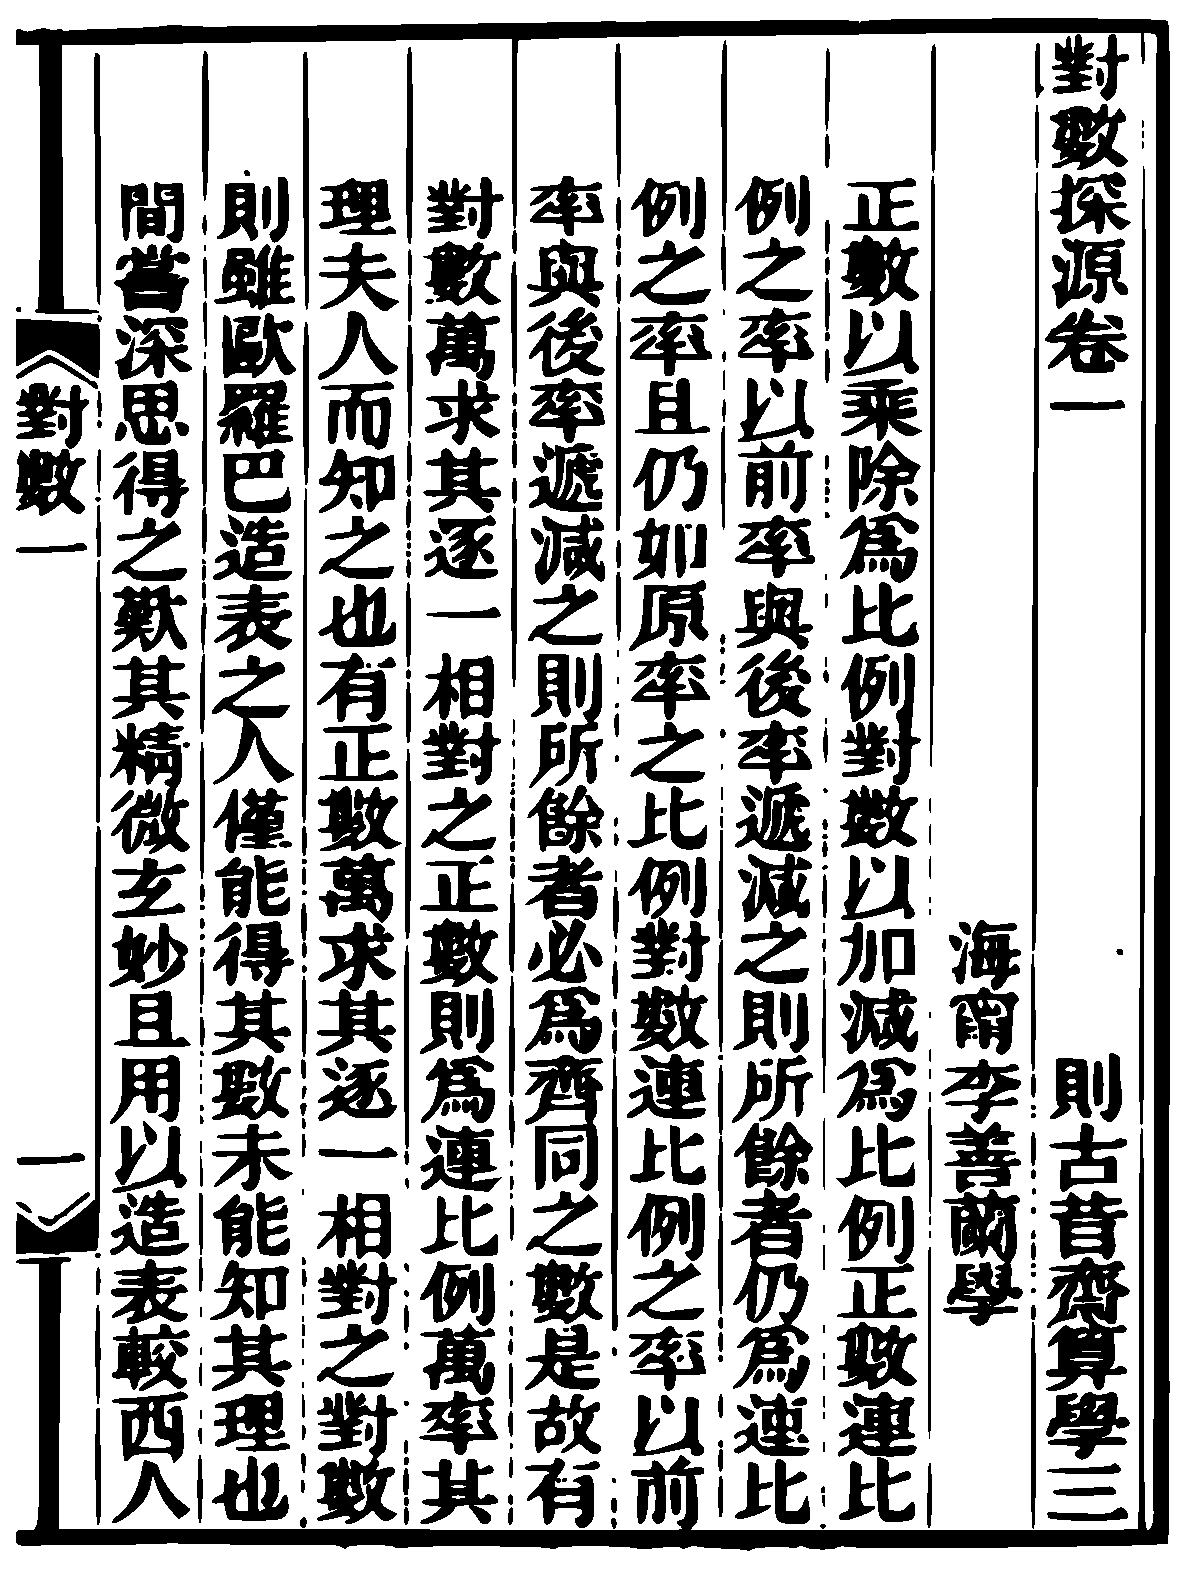
\includegraphics[width=8cm, height=10cm]{./Figs/suanxue.eps}
    \label{fig:suanxue}
    \caption{则古昔宅算学}
\end{figure}
\indent
1872年著《考數根法》,發表於《中西聞見錄》第二期,這是中算史上最早的一篇關於素數的論文。

\indent
在1852年-1866年,與偉烈亞力合譯《幾何原本》後9卷,完成明代利瑪竇、徐光啟未竟之業。

\indent
又與偉烈亞力、韋廉臣、艾約瑟合譯《談天》、《代數學》、《代微積拾級》
(美國伊萊亞斯·羅密士著)、《圓錐曲線說》、《奈端數理》、《重學》、《植物學》等書,
由墨海書館雕版刊行,對中國知識界有很大影響。


\section*{影響}

\indent
在1852年至1859年中,共譯書七、八部,計七、八十萬字,直接引進大量數學符號:
=、×、÷、<、>,而且他的翻譯工作具獨創性,創譯了許多數學名詞:代數、常數、
變數、已知數、函數、係數、指數、級數、單項式、多項式、微分、橫軸、縱軸、切線、
法線、曲線、漸近線、相似等,其他學科如:植物等,這些譯名獨具匠心,自然貼切,
其中許多譯名隨同他的譯著被引入日本,且沿用至今。

\begin{figure}[htbp]
    \centering
    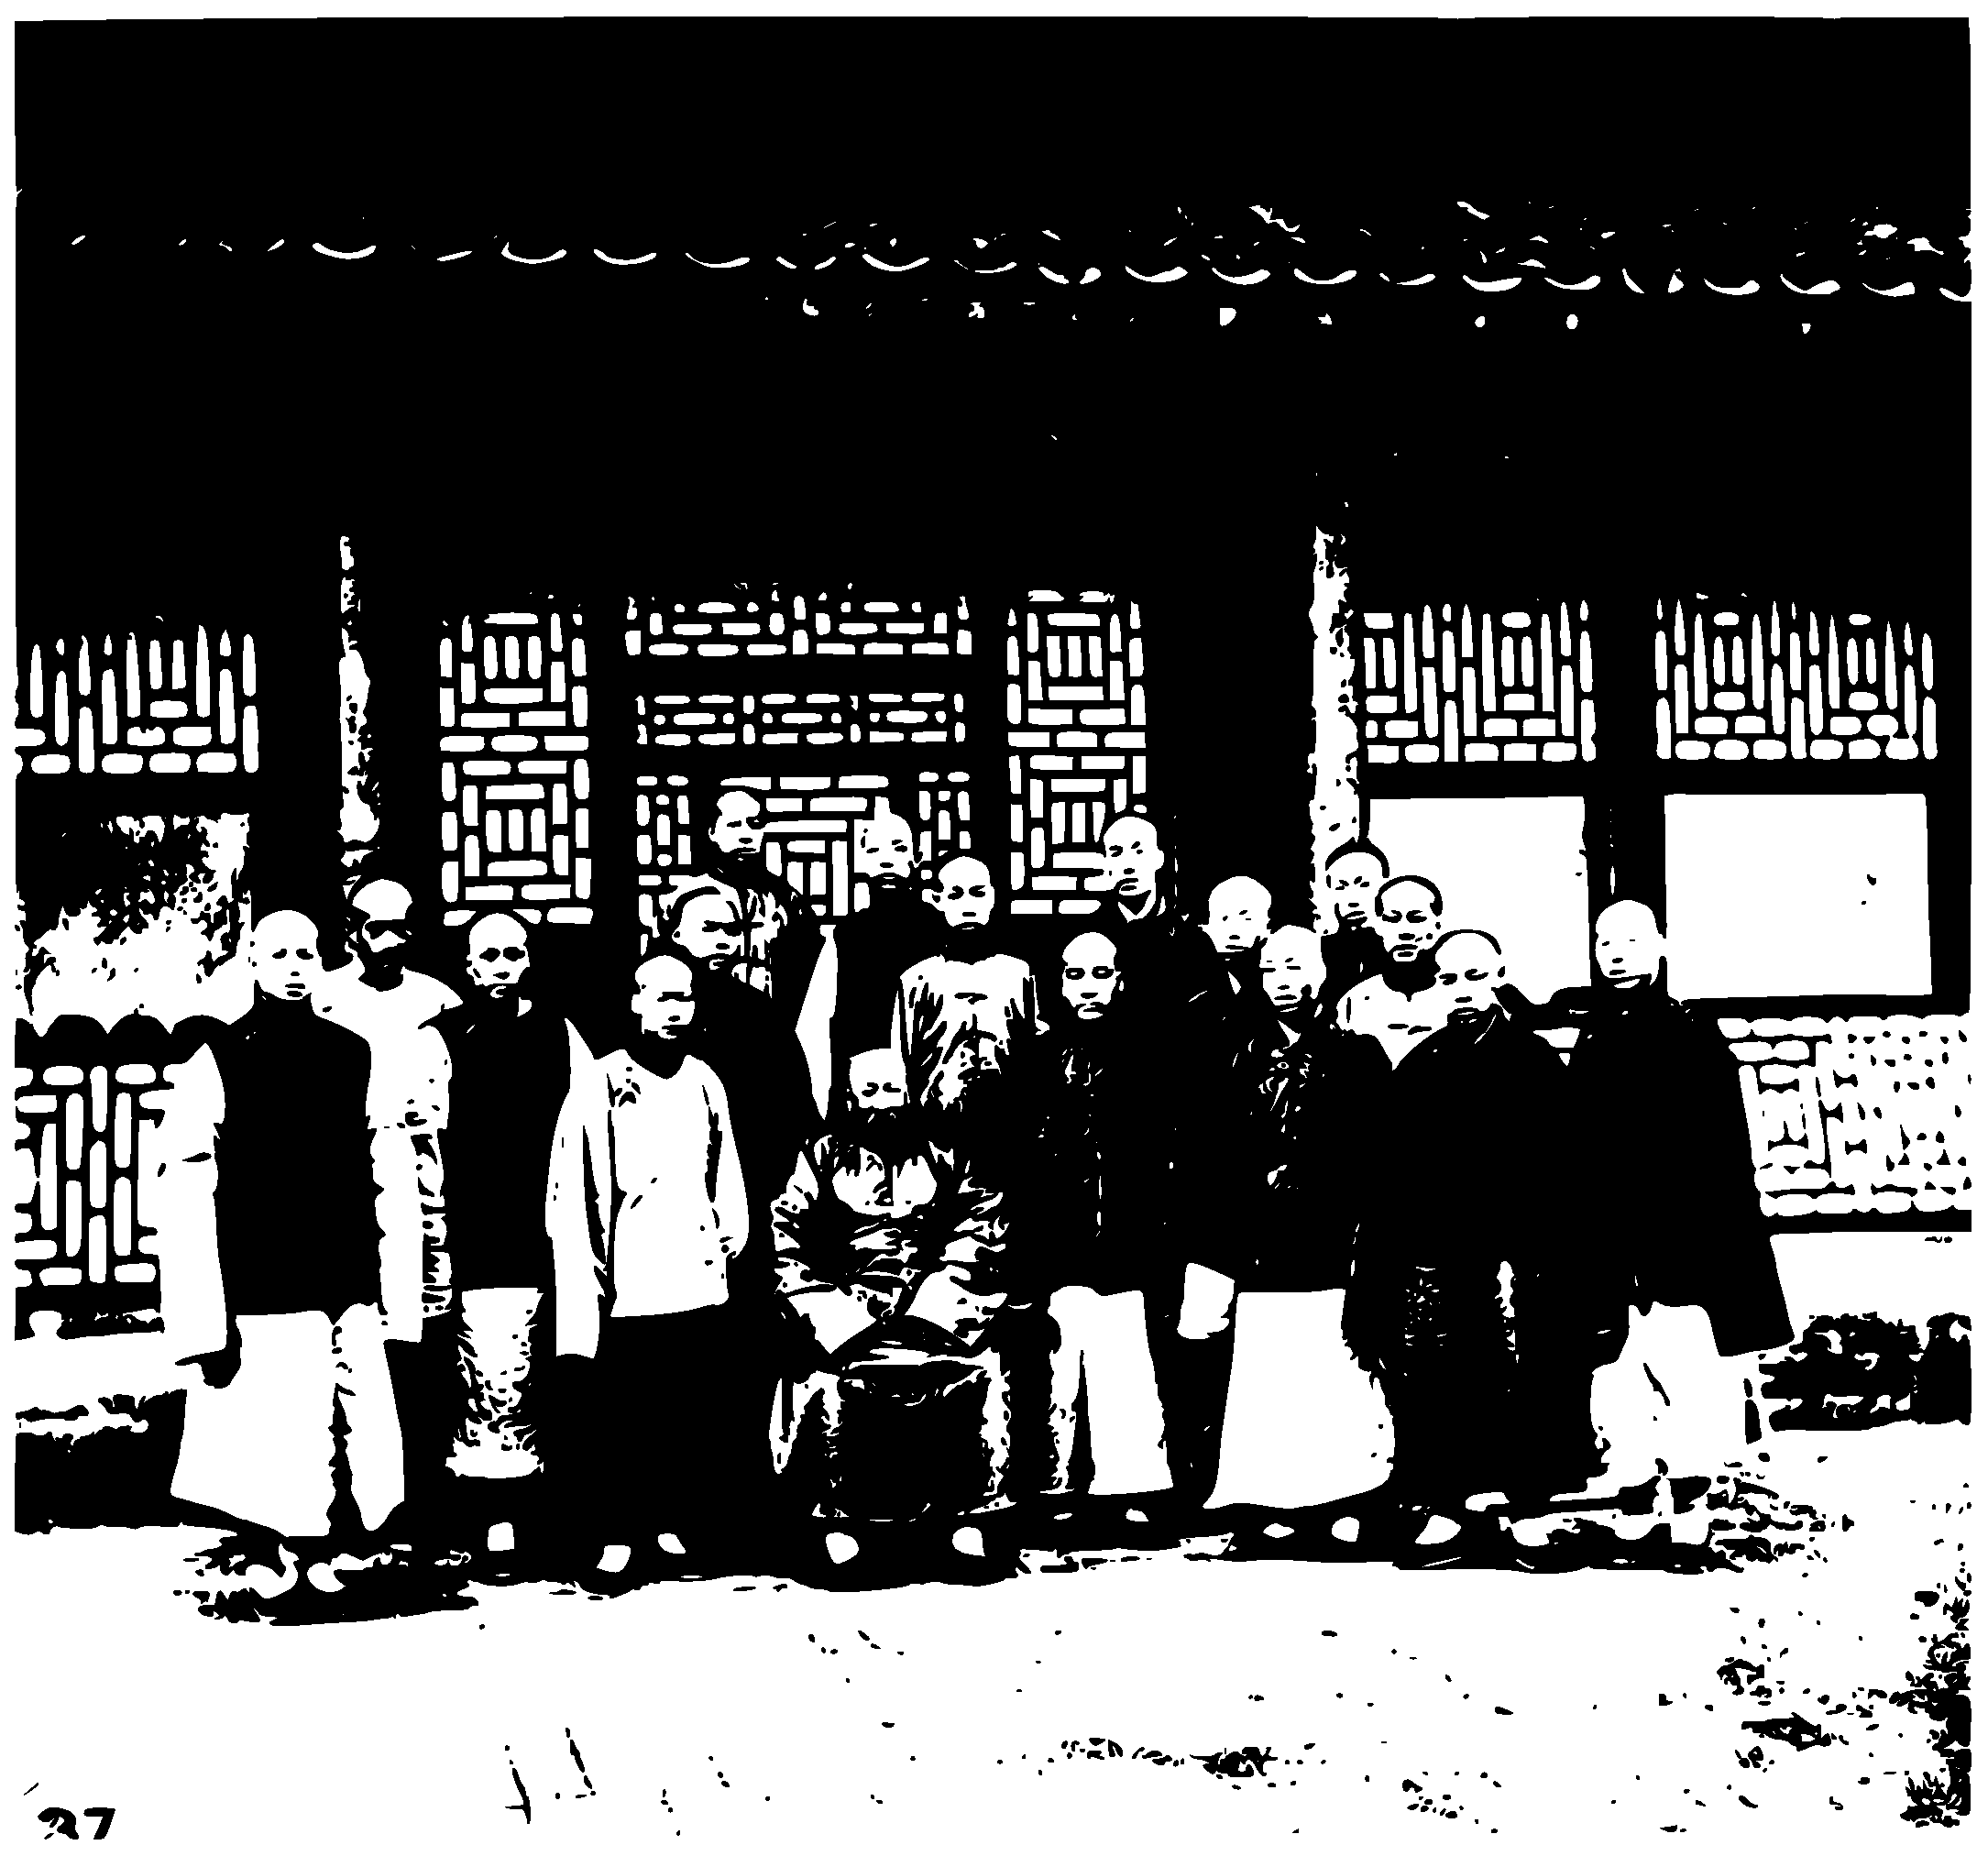
\includegraphics[width=12cm, height=10cm]{./Figs/LE-SHEN-LAN_AND_HIS_PUPILS.eps}
    \label{fig:Li_Shanlan_and_his_pupils}
    \caption{李善蘭和他的學生們}
\end{figure}

\end{CJK*}

\end{document}
